%%%%%%%%%%%%%%%%%%%%%%%%%%%%%%%%%%%%%%%%%%%%%%%%%%%%%%%%%%%%%%%%%%%%%%%%%%%%%%%%%%
\begin{frame}[fragile]\frametitle{}
\begin{center}
{\Large Summary: Checklist}

{\tiny (Ref: Building Yuki, A Level 3 Conversational AI Using Rasa 1.0 And Python For Beginners - Aditya Vivek Thota) }

\end{center}
\end{frame}


%%%%%%%%%%%%%%%%%%%%%%%%%%%%%%%%%%%%%%%%%%%%%%%%%%%%%%%%%%%
\begin{frame}\frametitle{Checkpoint 1: Understand What You Are Building}
Say, Objective: to build a Level 3 (??, find out more) chatbot. It can:
\begin{itemize}
\item can chitchat with you
\item can understand basic human phrases
\item can perform special actions
\item can autonomously complete a general conversation with a human
\item can store and retrieve information 
is deployed on Telegram, Slack, etc.
\end{itemize}
\end{frame}

%%%%%%%%%%%%%%%%%%%%%%%%%%%%%%%%%%%%%%%%%%%%%%%%%%%%%%%%%%%
\begin{frame}\frametitle{Checkpoint 2: Setting Up Your Development Environment}
\begin{itemize}
\item Anaconda Distribution For Python
\item Microsoft Visual C++ Redistributable (Prerequisite for Rasa Stack) 
\item Create a new virtual environment on Python 3.7 (not 2.*, or 3.6)
\item Install rasa, spacy and language models
\end{itemize}
\end{frame}

%%%%%%%%%%%%%%%%%%%%%%%%%%%%%%%%%%%%%%%%%%%%%%%%%%%%%%%%%%%
\begin{frame}\frametitle{Checkpoint 3: Creating The Skeleton Of Our Bot}
\begin{itemize}
\item Create a new folder; cd;
\item rasa init
\item Creates a default bot 
\item Work on top of this to build your own bot.
\end{itemize}
\end{frame}

%%%%%%%%%%%%%%%%%%%%%%%%%%%%%%%%%%%%%%%%%%%%%%%%%%%%%%%%%%%
\begin{frame}\frametitle{Checkpoint 4: Understanding The Structure Of Your Bot}
\begin{itemize}
\item ``data'' folder: Here lies your training data. You will find two files, nlu.md (training data to make the bot understand the human language) and stories.md (data to help the bot understand how to reply and what actions to take in a conversation).
\item ``models'' folder: Your trained models are saved  here.
\item ``actions.py'': defines all the custom functions, form actions, etc.
\item ``endpoints.yml'': URL to the place where the actions file is running
\item ``config.yml'': configuration parameters for pipeline and policies
\item ``credentials.yml'': access tokens and keys for external calls
\item ``domain.yml'': details of everything the bot is capable of
\end{itemize}
\end{frame}

%%%%%%%%%%%%%%%%%%%%%%%%%%%%%%%%%%%%%%%%%%%%%%%%%%%%%%%%%%%
\begin{frame}\frametitle{Checkpoint 5: Designing The User Experience (UX)}
List down all the functions/actions that the bot needs, to achieve its capabilities:
 \begin{itemize}
\item utter\_hello
\item handle\_out\_of\_scope
\item utter\_end
\item do\_rstaurant\_search (and so on \ldots)
\end{itemize}
\end{frame}

%%%%%%%%%%%%%%%%%%%%%%%%%%%%%%%%%%%%%%%%%%%%%%%%%%%%%%%%%%%
\begin{frame}\frametitle{Checkpoint 5: Designing The User Experience (UX)}
List of human intents the bot will have to detect from the messages users send it
 \begin{itemize}
\item greet
\item bye
\item restaurant\_search
\item affirm
\item deny
\item thank\_you
\item out\_of\_scope (everything else)
\end{itemize}
\end{frame}

%%%%%%%%%%%%%%%%%%%%%%%%%%%%%%%%%%%%%%%%%%%%%%%%%%%%%%%%%%%
\begin{frame}\frametitle{Checkpoint 5: Designing The User Experience (UX)}
Expand stories.md as needed. List possible user to interactions:
 \begin{itemize}
\item  happy path: the ideal expected scenario that happens when a user interacts with the bot
\item unhappy path (when user responds that answers are not correct)
\item Chit chat or small talk
\end{itemize}
\end{frame}

%%%%%%%%%%%%%%%%%%%%%%%%%%%%%%%%%%%%%%%%%%%%%%%%%%%%%%%%%%%
\begin{frame}\frametitle{Checkpoint 6: Building Your Rasa Model}
nlu.md
 \begin{itemize}
\item Some words in [] followed by (). 
\item These are [words] or expressions for the [entity] 
\item Rasa will classify intent and extract NER entities.
\end{itemize}

\end{frame}

%%%%%%%%%%%%%%%%%%%%%%%%%%%%%%%%%%%%%%%%%%%%%%%%%%%%%%%%%%%
\begin{frame}\frametitle{Checkpoint 7: Updating The Domain File}
domain.yml file must contain
 \begin{itemize}
\item Actions: names custom functions in actions.py as well as the ‘utter actions’
\item Entities
\item Intents
\item Forms
\item Slots
\item Templates
\end{itemize}
Highly functional AIs can have hundreds of actions, intents, entities and be connected to huge databases.
\end{frame}


%%%%%%%%%%%%%%%%%%%%%%%%%%%%%%%%%%%%%%%%%%%%%%%%%%%%%%%%%%%
\begin{frame}\frametitle{Checkpoint 8: Write Code For Your Custom Actions}
actions.py
 \begin{itemize}
\item Custom Actions, ie API calls
\item Form Actions
\item You must have a clear understanding of Requests library, JSON format, and how to extract what you want from the JSON payload in python.
\end{itemize}

\end{frame}

%%%%%%%%%%%%%%%%%%%%%%%%%%%%%%%%%%%%%%%%%%%%%%%%%%%%%%%%%%%
\begin{frame}\frametitle{Checkpoint 9: Updating The Config File}
config.yml
 \begin{itemize}
\item Configuring a Natural Language Understanding (NLU) pipeline consisting of various functions and extractors, through which the user input is passed through.
\item The outputs of this NLU pipeline is then passed on to a neural network that forms the Rasa Core.
\item Policies decide the next action (max confidence wins)
\end{itemize}

\end{frame}

%%%%%%%%%%%%%%%%%%%%%%%%%%%%%%%%%%%%%%%%%%%%%%%%%%%%%%%%%%%
\begin{frame}\frametitle{Checkpoint 10: Training/Running Your Bot}
 \begin{itemize}
\item To train both nlu and core models combined \lstinline|rasa train|
\item To run your bot in interactive Mode \lstinline|rasa interactive -m models --endpoint endpoints.yml| The interaction can be saved in stories
\item To run actions server:\lstinline|python -m rasa_sdk --actions actions|
\item To run locally (normal mode) \lstinline|rasa shell|
\item To run the bot on external channels (fb, telegram, etc) port number 80, \lstinline|rasa run -p 80|
\end{itemize}

\end{frame}

%%%%%%%%%%%%%%%%%%%%%%%%%%%%%%%%%%%%%%%%%%%%%%%%%%%%%%%%%%%
 \begin{frame}[fragile]\frametitle{And \ldots}

\begin{center}
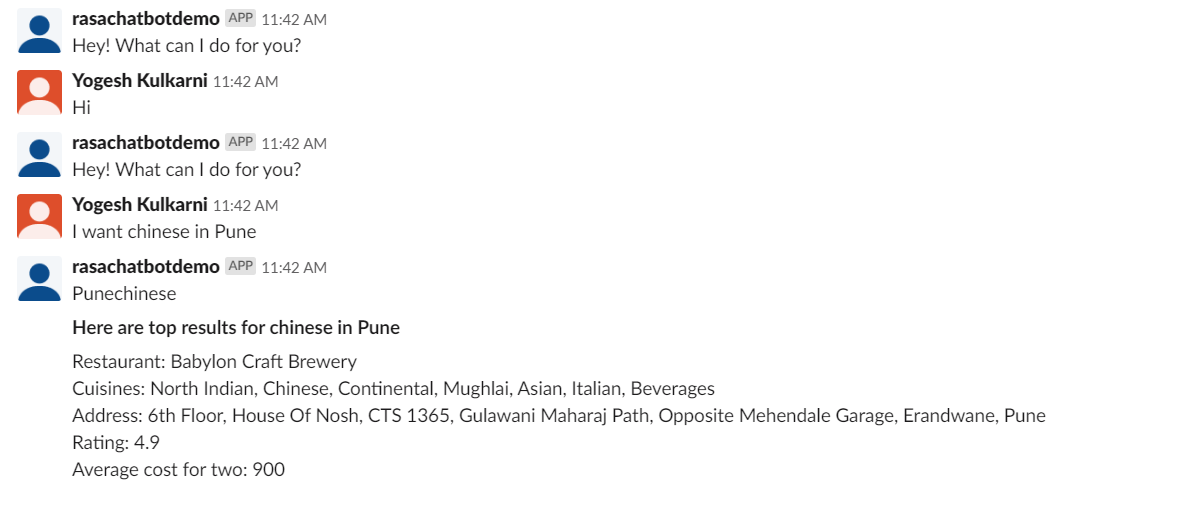
\includegraphics[width=\linewidth]{slackzomato}
\end{center}


\end{frame}
